
%% %-----Preámbulo ----- % % %

%Tipo de Documento: 
\documentclass{book} 

%Este paquete es utilizado para personalizar elementos por idioma: 
\usepackage[spanish ,mexico]{babel} 
  
%Este paquete es utilizado para la codificación de entrada: 
\usepackage[utf8]{inputenc} 

%Este paquete se utiliza para separar el texto en columnas
\usepackage{multicol}
\setlength{\columnseprule}{1pt}

%Paquete para fórmulas matemáticas
\usepackage{amssymb}

%Paquete para cargar gráficos
\usepackage{graphicx}

%Paquete para escribir tipo máquina de escribir
\usepackage{verbatim}

%Paquete para poner índice
\usepackage{makeidx}

%Otras declaraciones: 
\title{Don Quijote de la Mancha} 
\author{Sancho Panza} 


%%%---Cuerpo---%%%
\begin{document}
\maketitle

\chapter{Cervantes}
Miguel de Cervantes Saavedra\footnote{Alcal\'a de Henares, 29 de septiembre de 1547-Madrid, 22 de abril de 1616} fue un soldado, novelista, poeta y framaturgo espa\~nol.
Es considerado la m\'axima figura de la literatura espa\~nola y es universalmente conocido por haber escrito Don Quijote de la Mancha \ref{quijote} , que muchos cr\'iticos han descrito como la primera novela moderna y una de las mejores obras de la literatura universal, adem\'as de ser el libro m\'as editado y traducido de la historia, s\'olo superado por la Biblia.\\
\indent Una imagen de Cervantes mostrada en la figura \ref{cervantes}

\newpage
\begin{figure}[h]
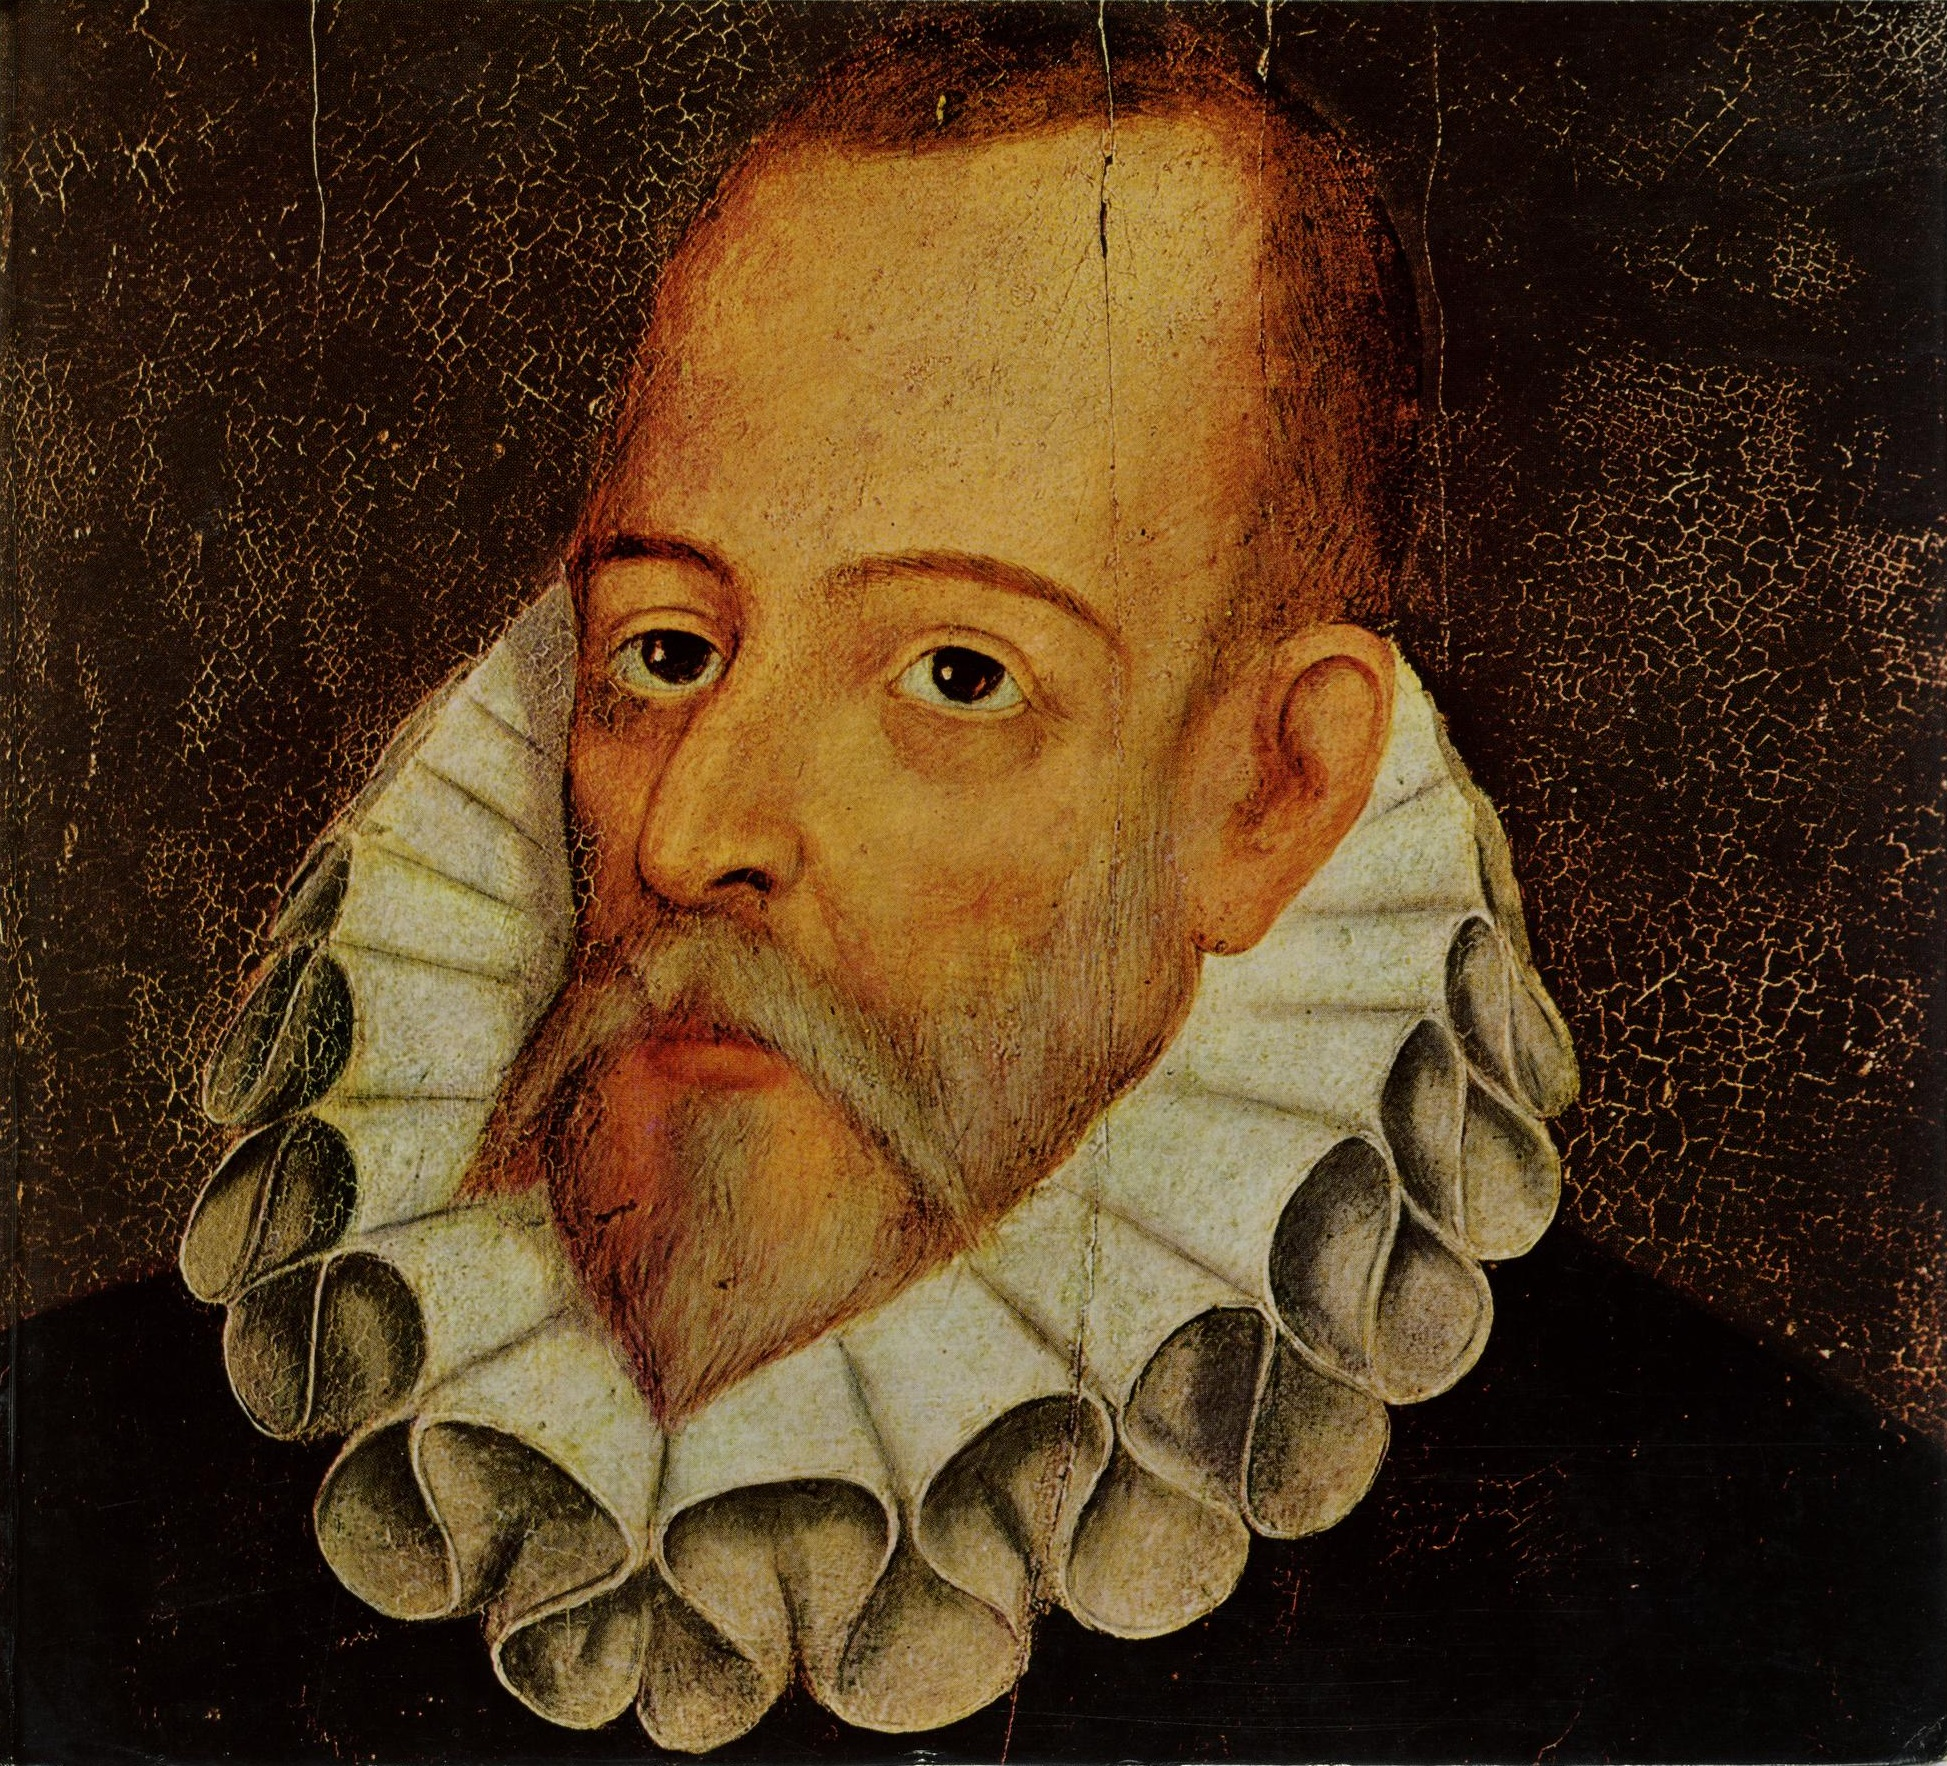
\includegraphics[scale=.2]{figCervantes}
\centering
\caption{Una imagen de Cervantes}
\label{cervantes}
\end{figure}


\chapter{Hablando de Don Quijote}
En cuanto a obra literaria, puede decirse que es la obra maestra de la literatura de humor de todos los tiempos. Adem\'as es la primera novela moderna y la primera novela polif\'onica, y ejercer\'a un influjo abrumador en toda la narrativa europea posterior.


\section{Un fragmento}
\begin{multicols}{3}
En un lugar de la Mancha, de cuyo nombre no quiero acordarme, no ha mucho tiempo que vivía un hidalgo de los de lanza en astillero, adarga antigua, rocín flaco y galgo corredor. Una olla de algo más vaca que carnero, salpicón las más noches, duelos y quebrantos los sábados, lentejas los viernes, algún palomino de añadidura los domingos,consumían las tres partes de su hacienda. El resto della concluían sayo de velarte, calzas de velludo para las fiestas con sus pantuflos de lo mismo, los días de entre semana se honraba con su vellori de lo más fino. 
\end{multicols}

\begin{figure}[t]
\centering
\begin{tabular}{cc}
\label{quijote}
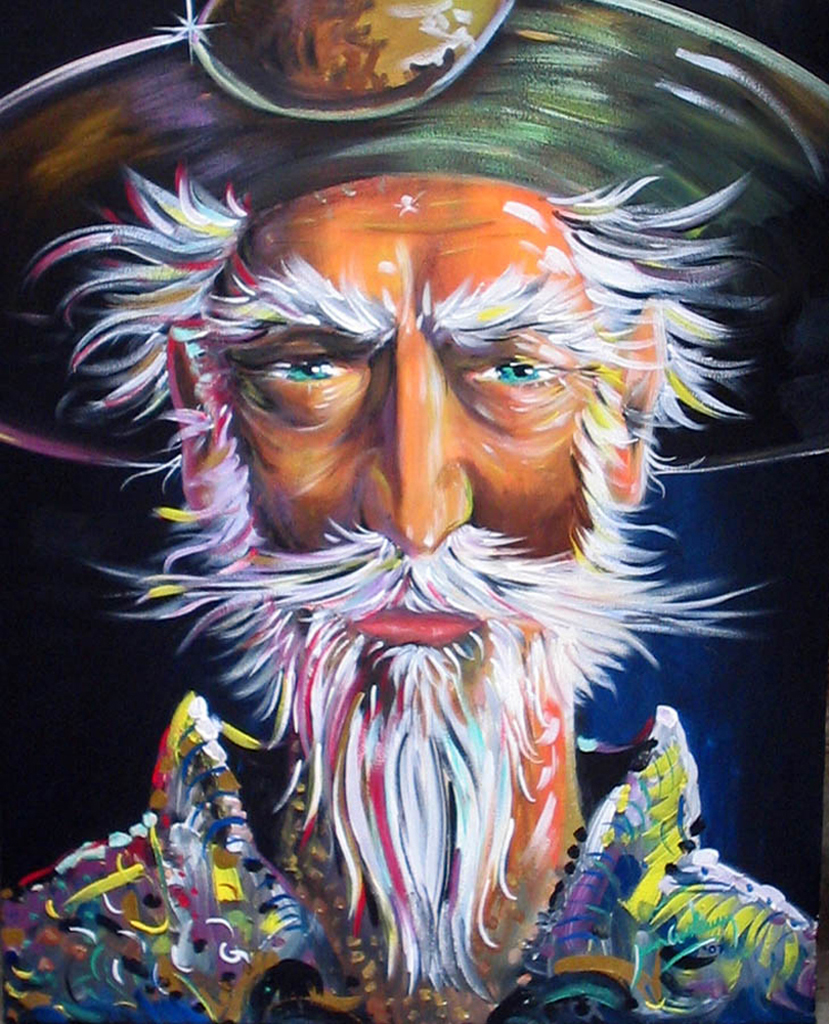
\includegraphics[scale=0.5, angle=60, trim={4cm 4cm 4cm 4cm}, clip]{quijote} & \qquad\qquad\qquad\qquad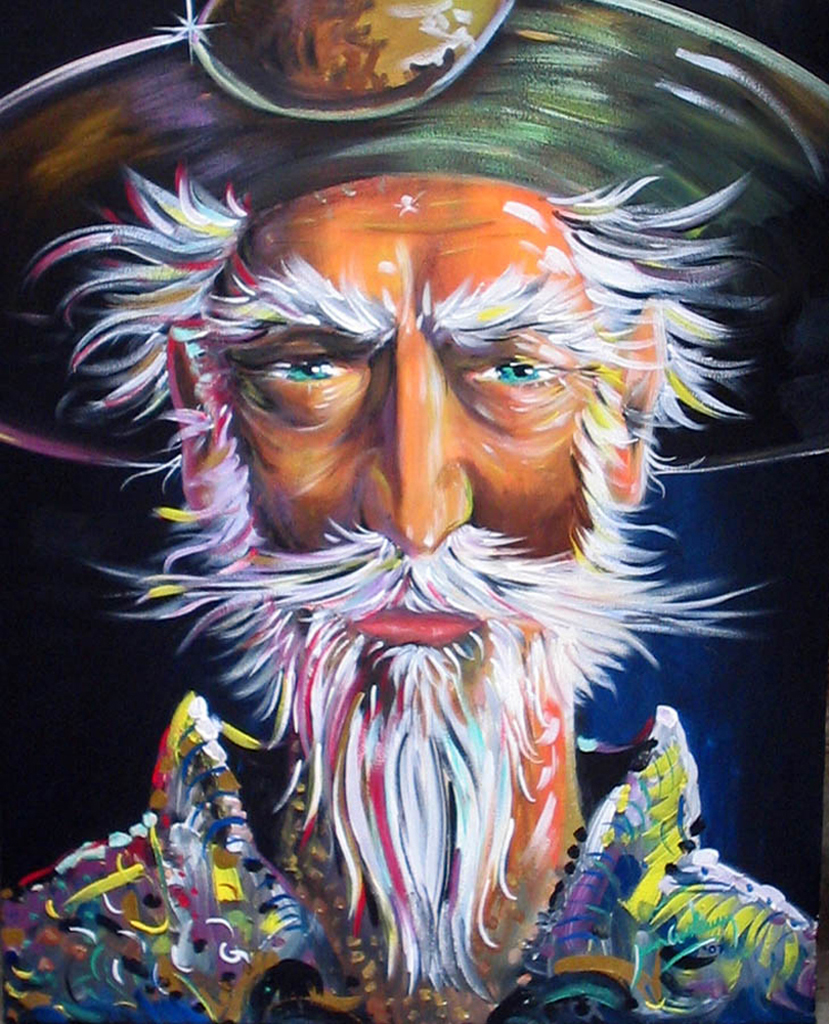
\includegraphics[scale=0.5, angle=40, trim={2cm 4cm 2cm 4cm}, clip]{quijote}
\end{tabular} 
\begin{tabular}{cc}
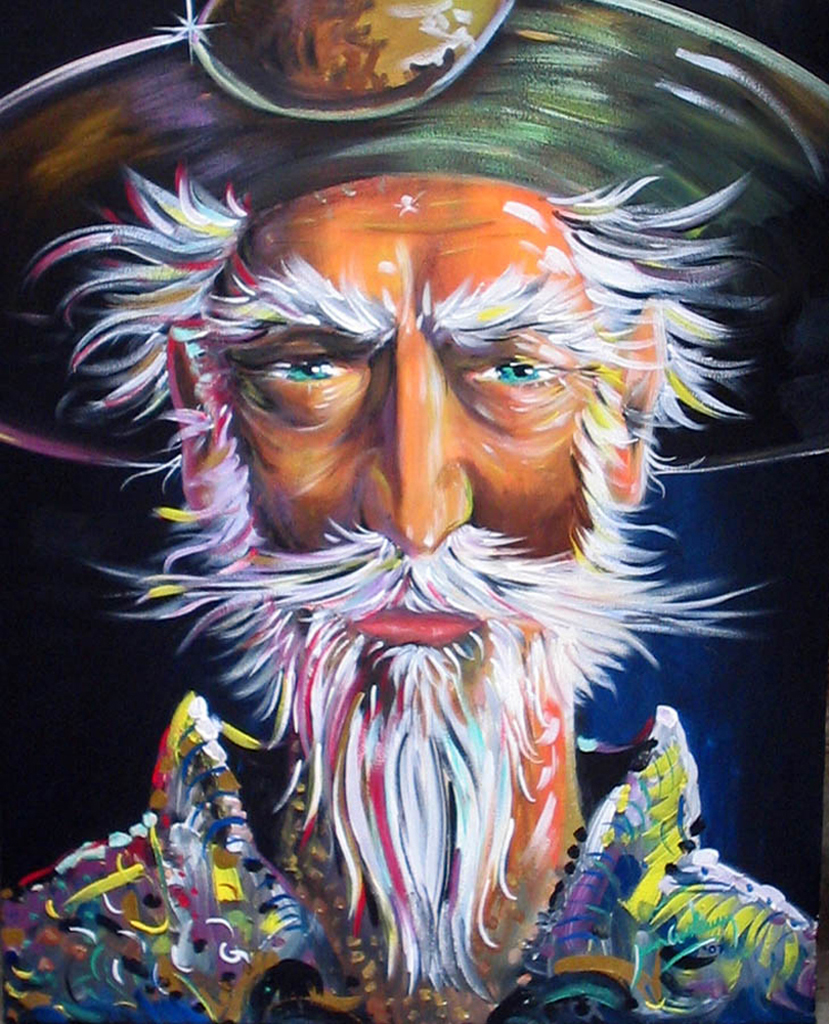
\includegraphics[scale=0.5, angle=-10]{quijote}&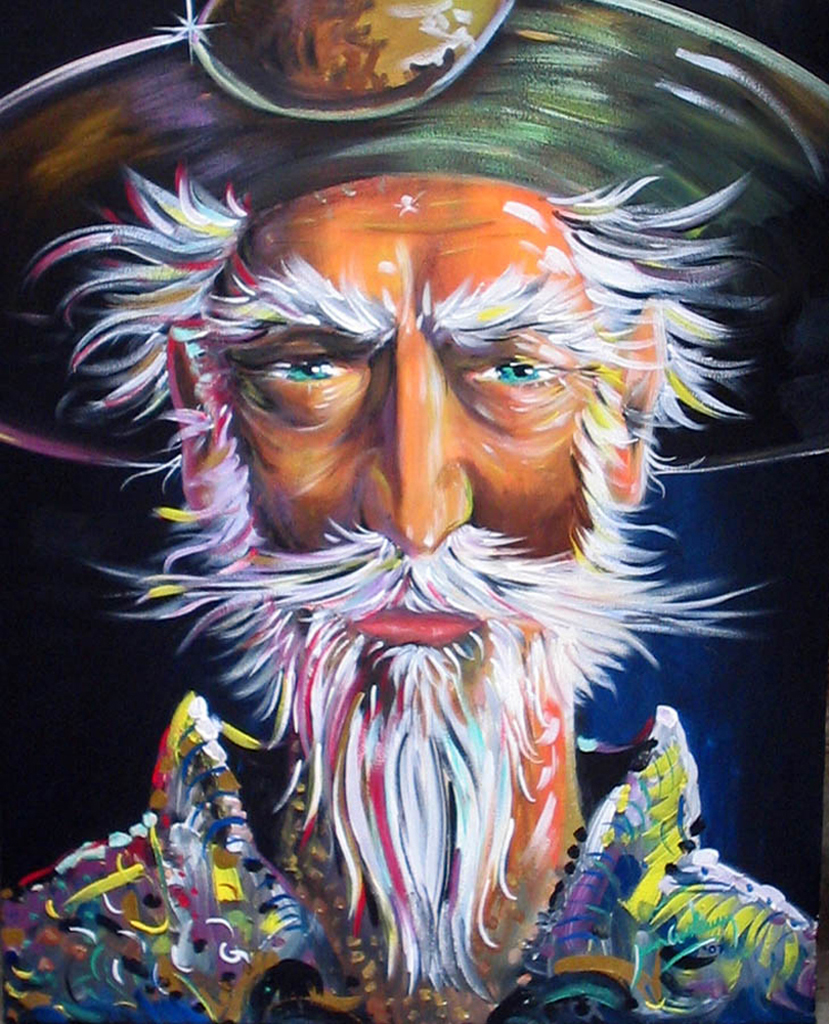
\includegraphics[scale=0.5, angle=20,trim={0cm 2cm 0cm 2cm}, clip]{quijote} 
\end{tabular}
\caption{El Quijote parece que est\'a dando vueltas}
\end{figure}

\end{document}
